\documentclass{article}
\usepackage[francais]{babel}
\usepackage[utf8]{inputenc}  
\usepackage[T1]{fontenc} 
\usepackage{multirow}
\usepackage{footnote}
\usepackage{longtable}
\usepackage{graphicx}

\title{Système Digital\\Rapport court microprossesseur}
\author{Elie Michel, Louis Garigue, Nicolas Jeannerod et Aurélien Delobelle}
\date{7 janvier 2013}

\begin{document}

\maketitle

\section{Introduction}

\paragraph{}
Nous avons commencé par nous baser sur le fonctionnement des microprocesseurs
MIPS étant donné que c'était la seule architecture que nous connaissions.
Nous avons cependant tenu à faire quelque chose de différent.

\paragraph{Ligne de conduite}
Notre premier choix important a été de décider que chaque fonction du
microprocesseur prendrait ses arguments dans les registres prévus à cet effet
(à savoir les \$a*), et renverrait ses résultats dans les registres prévus à
cet effet (les \$r*), à l'instar des appels système de MIPS qui regardent
toujours \$v0 et \$a0.

\paragraph{Densité}
Ce choix nous a dirigé vers un objectif de densité. Nous avons alors constaté
qu'il était possible de ne conserver que 4 registres
\footnote{\$a0, \$a1, \$r0, \$r1}, réduisant par là énormément le nombre
d'instructions de gestion de la mémoire, n'ayant plus besoin que de 2 bits
pour choisir un registre.

\paragraph{Pas si dense}
Nous avons au début cherché la densité maximale, avec un très petit jeu
d'instructions (sur 4 bits seulement !), réduit au minimum possible, mais
pour des raisons pratiques (pour que certaines manipulations ne prennent pas
trop d'instructions) nous l'avons enrichi. Finalement, les instructions sont
codées sur 6 bits.

\paragraph{}
C'est seulement en les rédigeant que nous avons fixé notre jeu d'instructions.

\section{Architecture générale}

\paragraph{Séparation en unités}
Nous avons séparé les instructions en 4 unités, les deux premiers bits
d'instructions gèrant l'appel de l'une d'elles :
\begin{itemize}
  \item SYS qui s'occupe des inputs et des outputs, au sens large (depuis
    l'horloge, et vers l'affichage).
  \item ALU qui fait les opérations de base, arithmétiques et logiques (add,
    sub, mult, div\footnote{La division est euclidienne} ; and, or, not, shift).
  \item MEM qui gère les accès mémoire, entre registres, et entre un registre
    et la RAM.
  \item JUMP qui contrôle l'adresse de lecture actuelle des instructions.
\end{itemize}

\paragraph{Inconvénients}
La séparation en quatre unité impose un nombre fixe d'instructions possibles
par unité, ce qui a amené quelques choix discutables :
\begin{itemize}
  \item Par manque de place, le move d'un \$a[i] vers un \$a[j]
    (resp. \$r[i] \$r[j]) n'existe pas.
  \item Nous avions absolument besoin du LI (load immediate), et ne trouvions
    pas de place pour cette instruction. Finalement, elle appartient à l'ALU.
  \item Pour certaines instructions, on ne peut regarder que dans \$a0 (et \$a1
    si deux arguments sont exigés), alors que pour d'autres on peut choisir
    le(s) registre(s) d'argument(s). Cela est dû au fait que certaines unités
    manquaient de place par rapport à d'autres.
  \item L'unité JUMP a accueilli les commandes WCA (Write Current Adress) et
    END (termine le programme)
\end{itemize}

\paragraph{Stockage de la date/heure}
Nous imaginions d'abord utiliser la RAM pour stocker les valeurs de la
date/heure, mais pour l'afficher, il aurait ensuite fallu lire 7 cases mémoires
différentes. Par soucis de rapidité, nous avons donc utilisé une mémoire
spécifique, ainsi la date/heure est affichée en une seule instruction.


\section{Architecture détaillée}

\paragraph{Le jeu d'instructions}~
\begin{savenotes}
\begin{longtable}{|l|l|}
  
  \hline
  Nom & Description \\
  \endfirsthead
  \hline
  Nom & Description \\
  \hline\hline
  \endhead


  \hline\hline
  \multicolumn{2}{|l|}{SYS} \\
  \hline
  INPUT  & \'Ecrit l'input dans un registre donné. \\
  OUTPUT & \'Ecrit le contenu de \$a0 dans la mémoire du timer. \\
  FLIP   & Actualise l'affichage du timer avec ce qu'il y a dans sa mémoire. \\
  
  \hline\hline
  \multicolumn{2}{|l|}{ALU} \\
  \hline
  \multicolumn{2}{|l|}{Arithmétique} \\
  \hline
  ADD   & Ajoute \$a0 et \$a1. Le résultat est dans \$r0, la retenue dans \$r1. \\
  SUB   & Soustrait \$a1 à \$a0. Le résultat est dans \$r0\footnote{$\$r0=\$a0-\$a1$ est certifié uniquement si $\$a0>\$a1$}, la retenue dans \$r1. \\
  MULT  & Multiplie \$a0 et \$a1. Le résultat est dans \$r0[0]...\$r0[n-1].\$r1[0]...\$r1[n-1].\\
  DIV   & Divise \$a0 par \$a1. Le quotient est dans \$r0, et le reste dans \$r1. \\
  \hline
  \multicolumn{2}{|l|}{Logique} \\
  \hline
  AND   & Calcule le AND bit-à-bit de \$a0 et \$a1 dans \$r0. \\
  OR    & Calcule le OR bit-à-bit de \$a0 et \$a1 dans \$r0. \\
  NOT   & Calcule le NOT bit-à-bit de \$a0 dans \$r0, et de \$a1 dans \$r1. \\
  SHIFT & SHIFT \$a0 de min(\$a1,n). \\
  \hline
  LI    & Charge une constante à trois bits\footnote{Le reste est rempli de 0} dans \$a0. \\
  
  \hline\hline
  \multicolumn{2}{|l|}{MEM} \\
  \hline
  \multirow{2}{*}{MOVE} & Déplace un \$a[i] vers un \$r[j]. \\
                        & Déplace un \$r[i] vers un \$a[j]. \\
  LOAD                  & Charge la valeur en RAM(\$r[i]) dans \$a[j]. \\
  SAVE                  & Enregistre la valeur \$a[i] dans RAM(\$r[j]). \\

  \hline\hline
  \multicolumn{2}{|l|}{JUMP} \\
  \hline
  JFRA & Augmente l'adresse de lecture (saut en avant relatif). \\
  JBRA & Diminue l'adresse de lecture (saut en arrière relatif). \\
  IIO  & Saute une instruction si le registre donné est nul. \\
  JAA  & Saut à une adresse absolue donnée par \$a0.\$a1 (ou \$r0.\$r1). \\
  WCA  & \'Ecriture de l'adresse courante dans \$a0.\$a1. \\
  END  & Termine le programme. \\
  \hline

\caption{Instructions microprocesseur}
\end{longtable}
\end{savenotes}

\paragraph{Interactions entre les différentes unités}~\\
On envoit à chaque unité son code opération (les quatre bits qui ne servent pas
à définir l'unité), et elle exécute cette opération. L'ALU par exemple, envoit
les valeurs \$a0 et \$a1 à chaque opérations, et reçoit tous les \$r0 et \$r1
associés. Elle mux alors selon le code opération qu'elle a reçu. De même, les
résultats des unités sont mux pour n'effectuer que l'action voulue. Selon
l'unité, ces résultats peuvent changer différents choses (les valeurs des
registres pour l'ALU, l'emplacement de la tête de lecture pour JUMP, etc).\\

\begin{figure}[h]
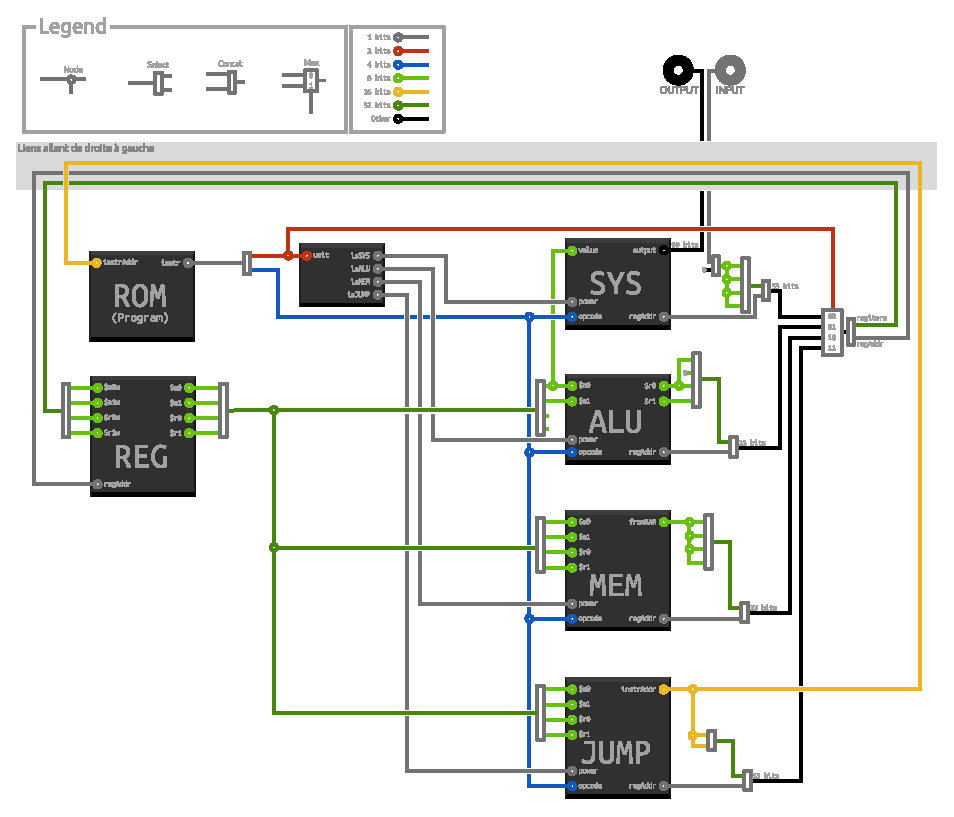
\includegraphics{archi.eps}
\caption{\label{archi} Architecture microprocesseur}
\end{figure}
La figure \ref{archi} présente l'architecture microprocesseur et l'interaction
entre les différentes unités.

\end{document}
